\documentclass[a4paper,twoside=false,abstract=false,numbers=noenddot,
titlepage=false,headings=small,parskip=half,version=last]{scrartcl}

\usepackage[utf8]{inputenc}
\usepackage[T1]{fontenc}
\usepackage[english]{babel}

\usepackage[colorlinks=true, pdfstartview=FitV,
linkcolor=black, citecolor=black, urlcolor=blue]{hyperref}
\usepackage{verbatim}
\usepackage{graphicx}
\usepackage{multirow}

\usepackage{tikz}
\usetikzlibrary{matrix}

\usepackage{amsmath}
\usepackage{amsthm}
\usepackage{amssymb}
\usepackage{amsfonts}

\theoremstyle{definition}
\newtheorem{exercise}{Exercise}

\theoremstyle{remark}
\newtheorem*{solution}{Solution}
\newtheorem*{remark}{Remark}

\newtheorem{theorem}{Theorem}[section]
\newtheorem{lemma}[theorem]{Lemma}
\newtheorem{proposition}[theorem]{Proposition}
\newtheorem{corollary}[theorem]{Corollary}

\newcommand{\NN}{\ensuremath{\mathbb{N}}}
\newcommand{\ZZ}{\ensuremath{\mathbb{Z}}}
\newcommand{\QQ}{\ensuremath{\mathbb{Q}}}
\newcommand{\RR}{\ensuremath{\mathbb{R}}}
\newcommand{\CC}{\ensuremath{\mathbb{C}}}
\newcommand{\GG}{\ensuremath{\mathcal{G}}}
\newcommand{\Fourier}{\ensuremath{\mathcal{F}}}
\newcommand{\Laplace}{\ensuremath{\mathcal{L}}}

\DeclareMathOperator{\Hom}{Hom}
\DeclareMathOperator{\End}{End}
\DeclareMathOperator{\im}{im}
\DeclareMathOperator{\id}{id}

\renewcommand{\labelenumi}{(\alph{enumi})}

\author{Jim Holmström - 890503-7571}
\title{Image Based Recognition and Classification - DD2427}
\subtitle{Excercise 5}

\begin{document}

\maketitle
\thispagestyle{empty}

\begin{exercise}
{\bf
    Show that the decision boundary induced by $1NN$ for the two feature vectors
    $\bar{x_1},\bar{x_2}$ is a straight line.
}
\end{exercise}
\begin{solution}
    Decision boundary is defined as: $|\bar{x_1}-\bar{x}|=|\bar{x_2}-\bar{x}|$
    since neither side can be negative we can simple square both side and expand
    the $L_2$-norm which gives us:\\

    $\sum{(x_{1,i}-x_i)^2}=\sum{(x_{2,i}-x_i)^2}$\\
    $\sum{x_{1,i}^2-2x_{1,i}x_i+x_i^2}=\sum{x_{2,i}^2-2x_{2,i}x_i+x_i^2}$\\
    $\sum{x_{1,i}^2-x_{2,i}^2+2(x_{2,i}-x_{1,i})x_i+0}=\sum{0}$\\
    $2\sum{(x_{2,i}-x_{1,i})x_i}+\sum{x_{1,i}^2-x_{2,i}^2}=0$\\
    $\sum{(x_{2,i}-x_{1,i})x_i}+\frac{\sum{x_{1,i}^2-x_{2,i}^2}}{2}=0$\\
    $\sum{c_ix_i}+d=0$

    With $c_i,d$ is all constants given $\bar{x_1},\bar{x_2}$, this is the form
    for multidimensional linear equation with an $(n-1)$-hyperplane as
    solution. $\qed$
\end{solution}
%-----------------------
\begin{exercise}
Draw decision boundaries for $1NN$-classifier with the training sets:\\
Class1:${(7, 11), (15, 9), (15, 7), (13, 5), (14, 4), (9, 3), (11, 3)}$\\
Class2:${(11, 11), (13, 11), (8, 10), (9, 9), (7, 7), (7, 5), (15, 3)}$\\
\end{exercise}
\begin{solution}
    \begin{center}
        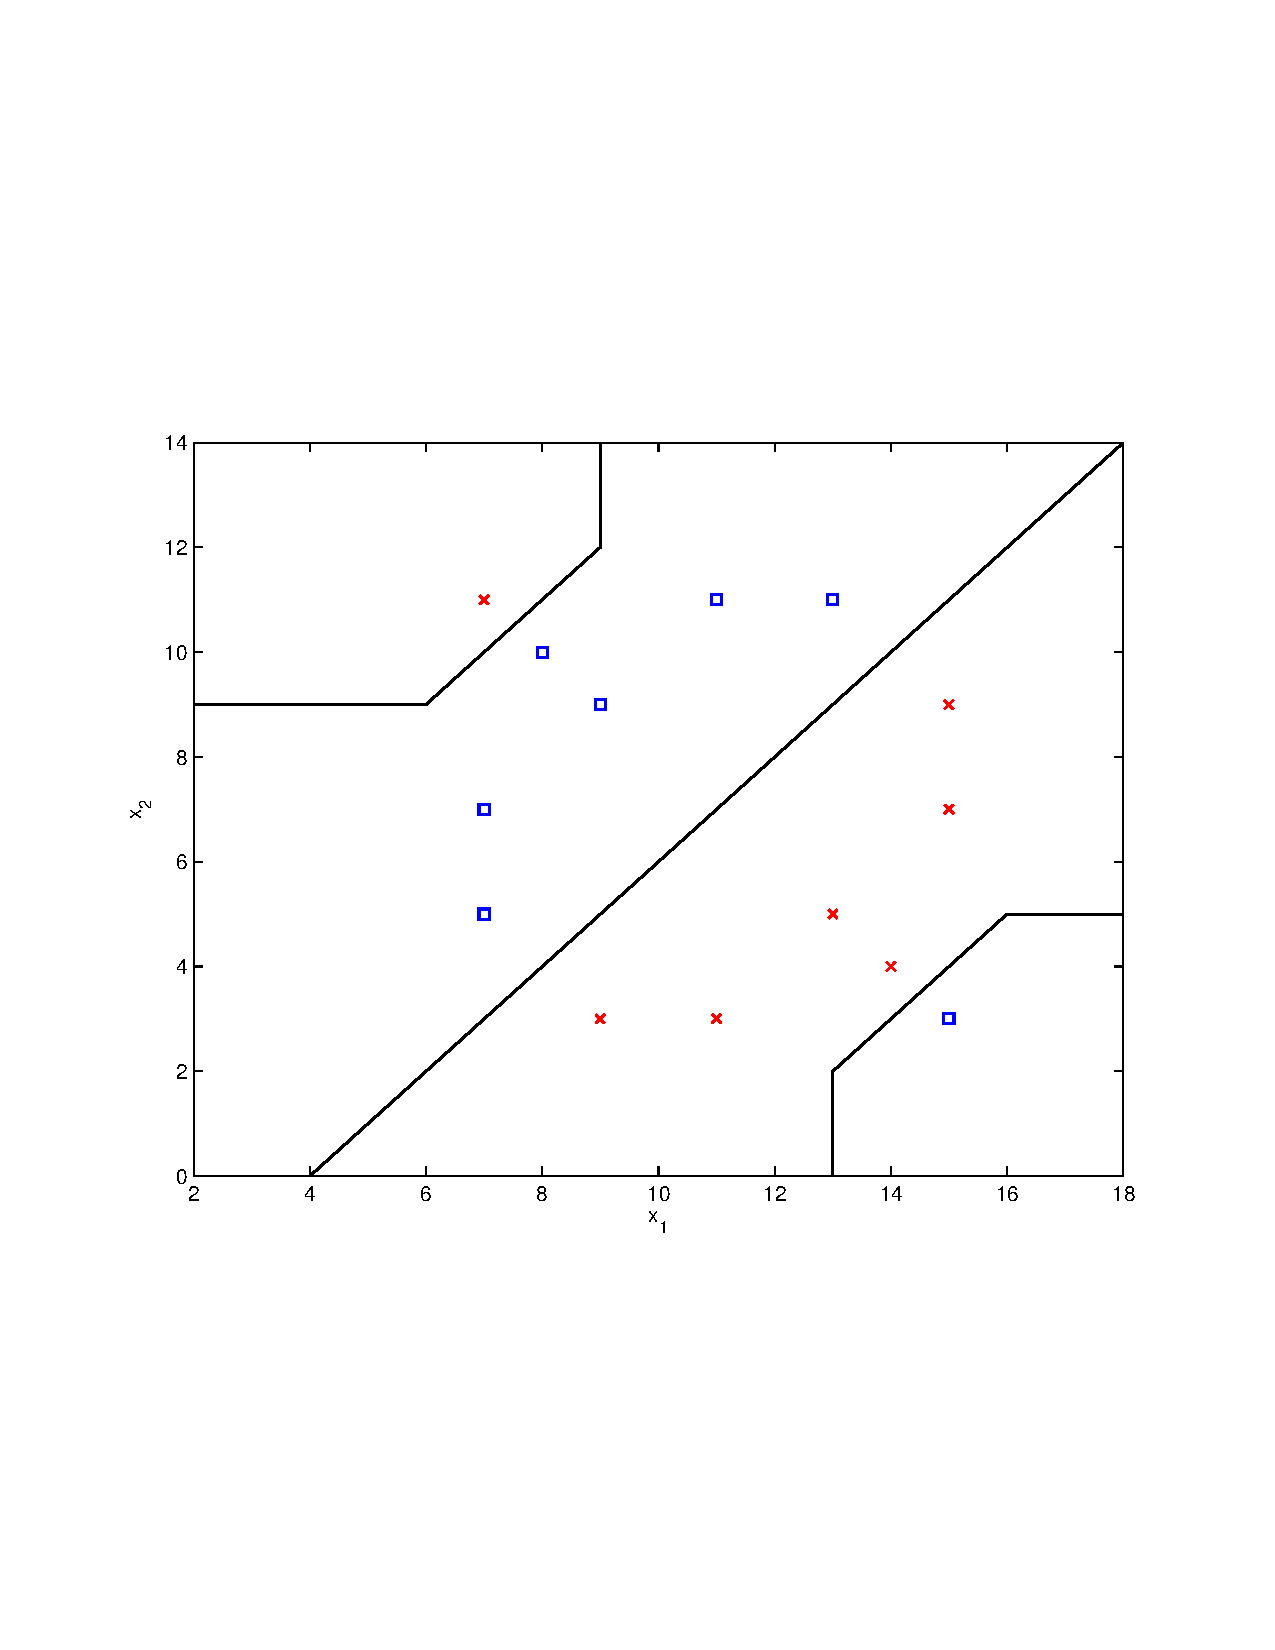
\includegraphics{exercise2.pdf}
    \end{center}
\end{solution}

\end{document}
